%!TEX root=../document.tex
\subsection{Hinzufügen von Benutzern und Benutzergruppen}
(Geschrieben von Dragana Sunaric)

\subsubsection{Erstellen der .ldif Files}
Die Nutzer können entweder über eine GUI wie beispielsweise \url{http://www.ldapadmin.org/} hinzugefügt werden oder über ein \textit{.ldif}-file in dem 
die Daten der einzelnen Benutzer und Benutzergruppen eingetragen werden.
Dieses File muss anschließend in den \textit{LDAP}-Verzeichnissdienst geladen werden.

Um eine Usergruppe hinzuzufügen muss folgendes in dem \textit{ldif}-file geschrieben werden :

\begin{lstlisting}[caption=Usergruppe hinzufügen]
dn: ou=People,dc=4chit,dc=at
objectClass: organizationalUnit
ou: People
\end{lstlisting}

hierbei haben wir die Usergruppe \textit{People} genannt und haben als domain den von uns zuvor gewählten \textit{domain-name}  \textit{4chit.at} geschrieben.

Um in dieser Usergruppe nun auch User anzulegen müssen wir diese User wie folgt erstellen:

\begin{lstlisting}[caption=User hinzufügen]
dn: uid=dsunaric,ou=People,dc=4chit,dc=at
objectClass: inetOrgPerson
objectClass: posixAccount
objectClass: shadowAccount
uid: dsunaric
sn: Draggy
givenName: Dragana
cn: Dragana.Sunaric
displayName: Dragana Sunaric
uidNumber: 10000
gidNumber: 5000
userPassword: 123456
gecos: dsunaric
loginShell: /bin/bash
homeDirectory: /home/dsunaric
\end{lstlisting}

Hierbei haben wir wieder bei den Usergruppen unseren \textit{domain-name} und sonstige metadaten zum Benutzer angegeben (Wie zum Beispiel die Usergruppe).

\textbf{Wichtig : es muss darauf geachtet werden, dass die uid und die uidNummer einzigartig ist}

Neben dem obenstehenden User haben wir noch 2 weitere hinzugefügt.
Das geschriebene File haben wir es unter dem Verzeichniss \textit{syt} unter dem Namen \textit{ldap\_4chit.ldif} gespeichert.

Um es in den \textit{lDAP}-Verzeichnissdienst zu laden müssen wir nun folgendes in die Konsole eingeben: 
\begin{center}
	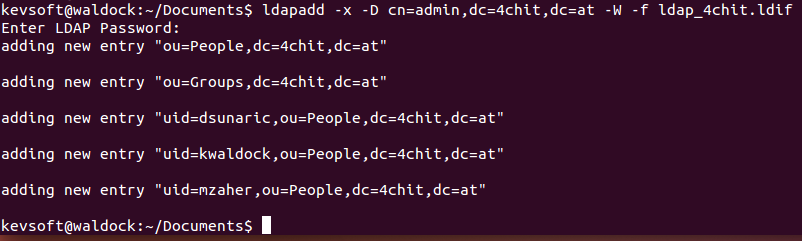
\includegraphics[width=1.0\linewidth]{images/a3_ldapadd.PNG}
\end{center}

Erfolgt die Ausgabe wie in unserem Beispiel verlief das Hinzufügen der Nutzer zumindest schon ohne Probleme.

Zu testzwecken haben wir noch einen \textit{LDAP}-search Befehl ausgeführt um zu testen ob die User tatsächlich angelegt sind:

\verb|ldapsearch -x -LLL -b dc=4chit,dc=at 'uid=dsunaric' cn gidNumber|

Nachdem der Befehl ausgeführt wurde sollten 3 Zeilen ausgegebenen werden. In der Untersten steht die \textit{gidNumber} (das Attribut nach dem wir gefiltert haben)